% \documentclass{book}

\documentclass[12pt]{article}
\usepackage[pdfborder={0 0 0.5 [3 2]}]{hyperref}%
\usepackage[left=1in,right=1in,top=1in,bottom=1in]{geometry}%
\usepackage[shortalphabetic]{amsrefs}%
\usepackage{amsmath}
\usepackage{enumerate}
\usepackage{enumitem}
\usepackage{amssymb}                
\usepackage{amsmath}                
\usepackage{amsfonts}
\usepackage{amsthm}
\usepackage{bbm}
\usepackage[table,xcdraw]{xcolor}
\usepackage{tikz}
\usepackage{float}
\usepackage{booktabs}
\usepackage{svg}
\usepackage{mathtools}
\usepackage{cool}
\usepackage{url}
\usepackage{graphicx,epsfig}
\usepackage{makecell}
\usepackage{array}

\graphicspath{ {images/} }

\def\noi{\noindent}
\def\T{{\mathbb T}}
\def\R{{\mathbb R}}
\def\N{{\mathbb N}}
\def\C{{\mathbb C}}
\def\Z{{\mathbb Z}}
\def\P{{\mathbb P}}
\def\E{{\mathbb E}}
\def\Q{\mathbb{Q}}
\def\ind{{\mathbb I}}

\begin{document}

\title{}
\author{\vspace{-10ex} }

\begin{center}
{\LARGE APMA 1650 -- Homework 6}\\
\vspace{5mm}
{\large Due Monday, July 25, 2016}\\
\vspace{5mm}
Homework is due during class or by 3:45 pm in the homework drop box in 182 George St.\\
Show all of your work used in deriving your solutions.
\end{center}

\begin{enumerate}

\item Suppose $X$ and $Y$ are discrete random variables with joint probability mass function given by:
\[
p(x, y) = \begin{cases}
\frac{1}{3} & (x, y) = (-1, 0), (0, 1), (1, 0) \\
\end{cases}
\]
(Recall that the discrete joint pmf specifies the probability for all pairs (x, y) which have positive probability. The three ordered pairs (x, y) above are the \emph{only} pairs (x,y) which have positive probability).
\begin{enumerate}
\item What is the covariance of $X$ and $Y$?
\item Are $X$ and $Y$ independent?
\end{enumerate}

\item Let $X$ be a binomial random variable with parameters $n$ and $p$. Consider the following estimator for $p$:
\[
\hat{p}_1 = \frac{X+1}{n+2}
\]
\begin{enumerate}
\item Find the bias of $\hat{p}_1$.
\item Find the mean square error (MSE) of $\hat{p}_1$.
\item The standard, unbiased estimator for $p$ is 
\[
\hat{p} = \frac{X}{n}
\]
We computed the MSE of $\hat{p}$ in class. Does the standard, unbiased estimator $\hat{p}$ always have a lower MSE than the biased estimator $\hat{p}_1$. In other words, can you find a value of $p$ for which $MSE(\hat{p}_1) < MSE(\hat{p})$? (If you don't want to do this for generic $n$, feel free to choose whatever value of $n$ you want).
\end{enumerate}

\item The reading on a voltmeter is uniformly distributed over the interval $[\theta, \theta+1]$, where $\theta$ is the true voltage of the circuit. Using your voltmeter, you take $n$ consecutive voltage readings $Y_1, \dots, Y_n$ from a single circuit.
\begin{enumerate}
\item Show that the sample mean $\bar{Y}$ is a biased estimator for $\theta$, and compute the bias of $\bar{Y}$.
\item Find a function of $\bar{Y}$ which is an unbiased estimator of $\theta$.
\item Find the MSE of $\bar{Y}$ (the biased estimator) when $\bar{Y}$ is used as an estimator of $\theta$.
\end{enumerate}

\item What do you know, another ACME widget factory question. In the last problem set, you had just launched a new line of MiniWidgets. In the intervening time, they have become so popular that your factory now has 10 machines devoted to producing MiniWidgets. The MiniWidgets produced by your machine have a mass which is normally distributed with a mean of 9 grams and a standard deviation of 0.2 grams.
\begin{enumerate}
\item On a routine inspection, you take a sample of 9 MiniWidgets produced by a single MiniWidget machine. You find that the average mass of the MiniWidgets in your sample is 8.85 grams. Do you think the MiniWidget machine is defective? (Hint: compute the probability that the sample mean is less than or equal to 8.85 grams).
\item On another inspection, you find a machine which appears to be defective. You want to know the mean mass of widgets produced by that machine (population mean $\mu$). To determine this, you take a sample of widgets from the machine and compute the sample mean $\bar{Y}$. Assume this machine produces widgets that are normally distributed, and that the standard deviation is the same as the other machines. How many widgets do you need to sample to be 95\% confident that the sample mean is within 0.05 grams of the true population mean?
\end{enumerate}

\item Take the unit circle (circle of radius 1) and inscribe it in a square. See the diagram below.

\begin{figure}[H]
\centering
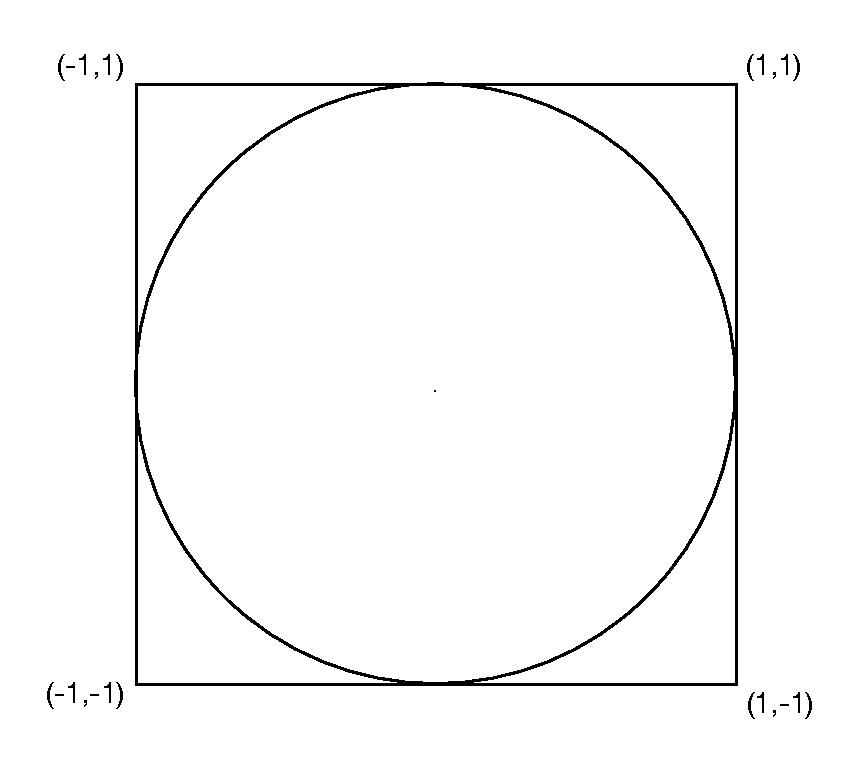
\includegraphics[width=6cm]{squarecircle.eps}
\end{figure}

You throw $n$ darts uniformly at random at the square. Let $Y$ be the number of darts which land in the circle. Form the estimator:
\[
\hat{\theta} = \frac{4Y}{n}
\]
What is the expected value of $\hat{\theta}$? What is $\hat{\theta}$ an estimator for?

\end{enumerate}

\end{document}

